\renewcommand{\arraystretch}{1.5}
\begin{longtable}{
    |p{4cm}
    |p{5cm}
    |p{5cm}|
}
\caption{Comparativa de sensores para medición de oxígeno disuelto.}
\label{tab:sensores_od} \\
\hline
\textbf{Característica} 
    & \textbf{Gravity: Analog Dissolved Oxygen Sensor (SEN0237) \cite{DFRobot_DO_Sensor}} 
    & \textbf{Atlas Scientific EZO-DO™ \cite{Atlas_DO_Sensor_Manual}} \\
\hline
\endfirsthead

\hline
\textbf{Característica} 
    & \textbf{Gravity: Analog Dissolved Oxygen Sensor (SEN0237) \cite{DFRobot_DO_Sensor}} 
    & \textbf{Atlas Scientific EZO-DO™ \cite{Atlas_DO_Sensor_Manual}} \\
\hline
\endhead

\hline
\multicolumn{3}{r}{\textit{Continúa en la siguiente página}} \\
\endfoot

\hline
\endlastfoot

Tipo de tecnología 
    & Galvánica 
    & Óptica \\ \hline

Rango de medición 
    & 0--20 mg/L 
    & 0--50 mg/L \\ \hline

Precisión 
    & $\pm$0.2 mg/L 
    & $\pm$0.05 mg/L \\ \hline

Tipo de salida 
    & Analógica (0--3.0 V) 
    & UART / I2C / Analógica \\ \hline

Voltaje de operación 
    & 3.3--5.5 V 
    & 3.3--5.5 V \\ \hline

Compatibilidad con ESP32 
    & Sí (ADC) 
    & Sí (UART/I2C/ADC) \\ \hline

Diseñado para monitoreo continuo 
    & No recomendado 
    & Sí \\ \hline

Vida útil de la sonda 
    & 6--12 meses 
    & $>$2 años \\ \hline

Calibración necesaria 
    & Frecuente 
    & Muy baja frecuencia \\ \hline

Costo aproximado 
    & \$169 USD 
    & \$195+ USD \\ \hline

Ventajas 
    & Bajo costo, fácil de usar 
    & Alta precisión, mínima deriva, muy estable \\ \hline

Desventajas 
    & Afectado por temperatura y flujo, no ideal para monitoreo 24/7 
    & Muy costoso, integración más compleja \\ \hline

Imagen
    & \shortstack{\\ 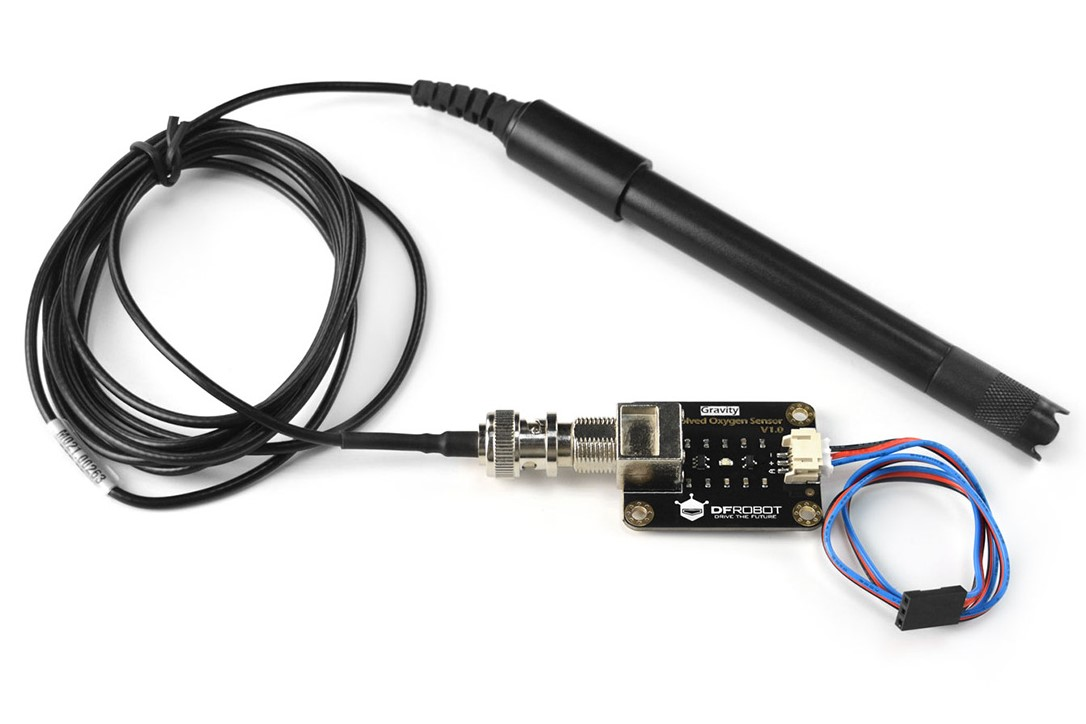
\includegraphics[width=0.8\linewidth]{Documento/Imagenes/Análisis/sensores/OD sensor.jpg}}
    & \shortstack{\\ 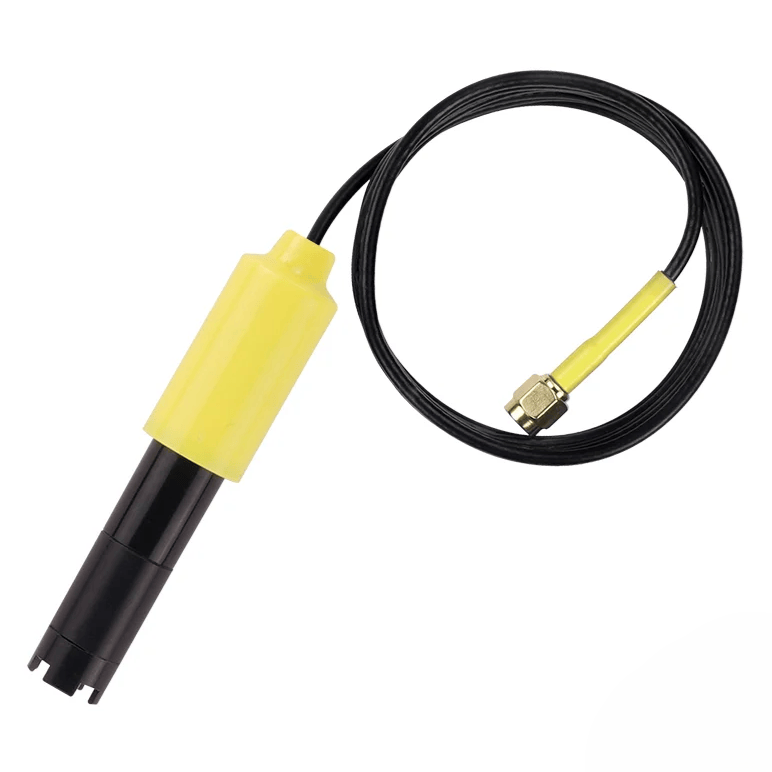
\includegraphics[width=0.8\linewidth]{Documento/Imagenes/Análisis/sensores/OD Atlas Sensor.png}} \\ \hline

\end{longtable}
